\documentclass[review]{elsarticle}

\usepackage{lineno,hyperref}
\usepackage{mathtools}
\usepackage[utf8]{inputenc}
\usepackage[english]{babel}
\DeclarePairedDelimiter{\ceil}{\lceil}{\rceil}
\modulolinenumbers[5]
\journal{Journal of \LaTeX\ Templates}

%%%%%%%%%%%%%%%%%%%%%%%
%% Elsevier bibliography styles
%%%%%%%%%%%%%%%%%%%%%%%
%% To change the style, put a % in front of the second line of the current style and
%% remove the % from the second line of the style you would like to use.
%%%%%%%%%%%%%%%%%%%%%%%

%% Numbered
%\bibliographystyle{model1-num-names}

%% Numbered without titles
%\bibliographystyle{model1a-num-names}

%% Harvard
%\bibliographystyle{model2-names.bst}\biboptions{authoryear}

%% Vancouver numbered
%\usepackage{numcompress}\bibliographystyle{model3-num-names}

%% Vancouver name/year
%\usepackage{numcompress}\bibliographystyle{model4-names}\biboptions{authoryear}

%% APA style
%\bibliographystyle{model5-names}\biboptions{authoryear}

%% AMA style
%\usepackage{numcompress}\bibliographystyle{model6-num-names}

%% `Elsevier LaTeX' style

\bibliographystyle{elsarticle-num}
%%%%%%%%%%%%%%%%%%%%%%%

\begin{document}

\begin{frontmatter}

\title{The 2-Dimensional Swept Rule Applied on Heterogeneous Architecture\tnoteref{mytitlenote}}
\tnotetext[mytitlenote]{Fully documented templates are available in the elsarticle package on \href{http://www.ctan.org/tex-archive/macros/latex/contrib/elsarticle}{CTAN}.}

%% Group authors per affiliation:
\author{Anthony Walker, Dr. Kyle Niemeyer\fnref{myfootnote}}
% \address{Radarweg 29, Amsterdam}
% \fntext[myfootnote]{Since 1880.}

%% or include affiliations in footnotes:
% \author[mymainaddress,mysecondaryaddress]{Elsevier Inc}
% \ead[url]{www.elsevier.com}

% \author[mysecondaryaddress]{Global Customer Service\corref{mycorrespondingauthor}}
% \cortext[mycorrespondingauthor]{Corresponding author}
% \ead{walkanth@oregonstate.edu}
%
% \address[mymainaddress]{1600 John F Kennedy Boulevard, Philadelphia}
% \address[mysecondaryaddress]{360 Park Avenue South, New York}

\begin{abstract}
This paper contain is a study of the swept rule in two dimensions on heterogeneous
architecture.
\end{abstract}

\begin{keyword}
\texttt{elsarticle.cls}\sep \LaTeX\sep Elsevier \sep template
\MSC[2010] 00-01\sep  99-00
\end{keyword}

\end{frontmatter}

\linenumbers

you can do something like:
1. solving multidimensional PDEs for practical problems requires using shared and/or distributed memory systems
2.  bandwidth and latency between processing units, particularly in distributed systems, can be a bottleneck. separately (but related), when you have things like GPUs, you want to do as much local work as possible before communicating between the independent processors
3. how have others tried to solve this?
4. what past work has been done specifically on the swept approach?
5. what are the objectives of this study?

\section{Introduction}

Unsteady multidimensional PDES often require the use of shared and/or distributed memory systems to obtain a solution with practical grid resolution or scale in a reasonable time frame. The solution of many problems at any point in the grid is inherently dependent on the neighboring points in each dimension. This dependence necessitates communication between computing nodes. Each of these communications incurs a minimum cost regardless of the amount of information communicated known as network latency. On the contrary, bandwidth is the variable cost associated with the amount of data transferred. This latency can be significantly restrictive on the solution's time to completion, especially when using distributed systems. This barrier to scaling is referred to as the latency barrier and is particularly impactful in large scale simulations advancing many time steps (i.e. ones that requires a large amount of communication) \cite{Alhubail2016ThePDEs}. The barrier is bottle neck in the system which can limit the performance regardless of the architecture.

\par
From the architecture perspective, GPU can be incredibly powerful when utilized in scientific computing. GPUs also perform best when as much work as possible is completed locally prior to communication. [ADD MORE HERE, READ DANS PAPER AND MOTIVATION ON GPUS]

\par This issue has been approached in many ways. The most closely related to this study is the swept rule which was first implemented by Alhubail et al. in \cite{Alhubail2016ThePDEs}. This technique is closely related to cache optimization techniques, parallel-in-time methods, and communication avoidance (CA) algorithms but there are technical differences in each of the strategies.

\par
Parallel-in-time methods differ from the swept rule in the sense that it is not iterative.

\par
Cache optimization techniques differ from the swept rule as the intention is not to stop communication but optimize it.

\par
The swept rule differs from communication avoidance techniques in as it does not directly involve overlapping parts of the communication.

\par
In this paper, PySweep, a 2 dimensional PDE solver was implemented and tested on heterogeneous (i.e. utilizes both a CPU and GPU) architecture. This solver is openly available on GitHub at \textit{https://github.com/walkanth/pysweep}. This differs from past work in a few ways. The swept rule was originally developed by Alhubail et al. who published a 1 dimensional CPU only swept PDE solver which was tested by solving the Kuramoto-Sivashinsky equation and the compressible Euler equations. They concluded that in each case a number of integrations can be performed during the latency time of a communication. Their analysis shows that integration can be made faster by latency reduction and increasing computing power of the computing nodes \cite{Alhubail2016ThePDEs}. Alhubail et al. followed this work with a 2 dimensional CPU only swept PDE solver which reported speed ups of up to 3 times compared to classical methods when solving the Wave and Euler equations \cite{Alhubail2018ThePDEs}. These studies differ from this study and PySweep in multiple ways. The most prominent are the dimensionality and intended architecture.
\par
Magee et al. created multiple 1 dimensional PDE solvers which includes GPU only and heterogeneous solvers. It was concluded that their shared memory approach typically performed better than alternative approaches. This study solved the compressible Euler equations were solved as done by Alhubail et al. \cite{Alhubail2016ThePDEs} but speed up was not obtained in all cases. This is attributed to greater usage of lower level memory and limits performance benefits of the swept rule depending on the problem \cite{Magee2018AcceleratingDecomposition}. As this study is an extension of Magee et al.'s work, it differs in mainly the dimensionality. The implementation of PySweep does utilize and extend some of the implementation strategies that showed promise in the aforementioned study.

\par
The objective of this study are to implement the swept rule in 2 dimensions on heterogeneous architecture and study the performance capabilities of such a solver based on system parameters. The first parameter of interest in the block size Magee et al. showed a dependence on the block size so it is of interest to determine the change in behavior when added another dimension which the solvers are not identical, the theory is the same and comparison can provide valuable insight into the effects of the extra dimension. Magee et al. likewise showed a performance dependence on the GPU affinity, Array size, and [READ PAPERS].

\par
The effect of added dimensionality on these parameters is a pragmatic interest and can be considered from multiple perspectives. The primary objective is speed up of simulations requiring high performance computing (HPC) through the reduction of network latency. The swept rule is motivated by improved time to solutions of problems involving complicated phenomena frequently requiring the use of HPC systems. While many simplifications exist to reduce the dimensionality of these problems, the most practical approach is what is experienced in reality which is 3 dimensions. While this solver is not 3 dimensional, it is a step in that direction which can provide insight to the performance of the swept rule in multiple dimensions. In the case of this specific solver, it can provide insight to the performance of the heterogeneous solver in 2 dimensions that employ this latency reduction technique. This insight can offer the chance to optimize system usage and promote faster design and prototype of the aforementioned applications.

\par
In the event that time is not the primary concern, available resources or resource costs are other important considerations. The ability to execute a simulation on a HPC system is dependent on access to such systems. In the case of Amazon EC2, simulation time can be purchased at different hourly rates depending on the application. This can quickly become expensive for applications that require large numbers of computing hours. Network latency is maximized in applications requiring a lot of communication because each communication takes a finite amount of time regardless of the data size. However, that does not mean that improvement cannot be obtained on smaller systems. This claim is supported by findings from Magee et al. as they tested their code on a work station with a single GPU and CPU and obtained speed up \cite{Magee2018AcceleratingDecomposition}. While this is not the primary focus, an optimized solver that reduces latency would require less computing resources and more practical applications could potentially be solved on smaller less costly computing clusters.

\par
Hopefully, it is clear at this point that latency reduction is important in high performance computing and scientific applications from multiple perspectives as this is the intention of this work. The work in this paper is presented in a traditional manner as follows. The implementation of the swept rule will be discussed along with the design decisions, strategies applied, and restrictions with respect to this specific code. The testing procedure and guidelines for code usage will be presented. The results of testing the solver will be discussed. Finally, the paper will close with conclusions and recommended future work.

%
%  Implementation
%

\section{Implementation}
The implementation of the 2D swept rule on heterogeneous architecture, referred to as PySweep on GitHub, involves multiple languages, architectures, strategies, and problems which will be discussed along with decisions made during the implementation process. This solver is also paired with a more traditional (standard) solver that communicates as is necessary to complete a step. This standard solver is also avaliable in the repository for comparison. The code was developed on a workstation with 2 Nvidia GPUs (Tesla K40c and Quadro K620) and a CPU with 16 cores. It was tested on a small computing cluster at Oregon State University which includes a single Nvidia Tesla K40m and 6 Intel(R) Xeon(R) CPU E5-2660 v3 CPUs which are linked via InfiniBand.

\par
PySweep was implemented primarily in python as it is a simple yet powerful high level programming language that has a multitude of open source packages used for scientific computing and is frequently used for such applications. There is also a well known GPU computing package, PyCuda, that provides a simple interface for working with Nvidia GPUs \cite{KlocknerPyCUDAGeneration}. The GPU kernels were specifically written in CUDA in lieu of using python abstractions as the abstractions tended to display decreased performance. It is believed that this slowdown is caused by more frequent communication with the CPU. Since a major part of the study was speed improvement through reduced communication, it was appropriate to write kernels in CUDA. 

\par
The CPU parallelism was implemented with a combination of mpi4py, a MPI (Message Passing Interface) package for python, and python's built-in multiprocessing module --- so the code can operate on distributed computing systems. A MPI process that controls the behavior of it's respective device is spawned for each GPU and the CPU. The CPU's MPI process will spawn sub-processes based on available resources to fully utilize the CPU. A complete list of the packages used can be found in the PySweep repository.

\par Domain decomposition, process handling, and work allocation must occur prior to the beginning of the solution process. The swept solver and standard solver both use the same decomposition, process handling, and work allocation strategies so that the performance comparison between the two is representative of the differences between the solvers. The swept solver does have some additional calculations prior to solving which are necessary for the swept solution process. These additional calculations are penalties of this swept implementation which may affect the performance. 

\par
There are 4 phases that occur during the swept solution process. In the code, these phases are referred to as UpPyramid, Bridge (X or Y), Octahedron, and DownPyramid so that convention will be continued here. They are so named as these shapes are produced during the solution procedure if you visual the solution's progression in 3 dimensions (x,y,t); this will be demonstrated in later figures for a general case. However, the specific shape that forms in each phase is a function of the spatial stencil and time scheme chosen to solve a given problem.  

\par
The numerical scheme in both space and time directly affects the performance of the swept rule as it limits the number of steps that can be taken per phase. PySweep was implemented with only symmetrical stencils on a structured grid for simplicity. So, lets define the number of points on each side of the current point as $n$. The height $h$ of each phase except the Octahedron---or number of steps in time---is then
\begin{equation}
    h = \bigg(\frac{b}{2n}-1\bigg)
\end{equation}
for a given block size $b$. The height of the Octahedron is $2h$. This height is effectively reduced by the number of intermediate steps required by the temporal scheme e.g. if a second order Runge-Kutta is used in time then the effective height is $h/2$ because RK2 takes two intermediate steps. This is not necessarily detrimental to performance as a typical solver is subjected to more communications in this case as well.

\par
The block size is a parameter which determines how many threads will be executed in a group referred to as a block. This parameter plays a role in the performance of the swept rule on heterogeneous architecture as it directly limits the number of steps that can be taken by any swept phase. The block size is restricted by both the code and the hardware used. The workstation GPU, a Tesla K40c, restricts blocks to a maximum of $1024$ threads per block ($T_{max}$).
The block size, $b$, is then restricted by the code to being square i.e. the x and y dimension of the block must be the same. This was done because the number of steps taken in time via the swept rule is directly limited by the minimum dimension of the block. The block is finally limited by the expression
\begin{equation}
    b  = (2nf)^2,
\end{equation}
where $f$ is any positive integer such that $(2n+1)^2 < b < T_{max}$ and $n$ is as previously described. In the former example,
\begin{equation}
  \ceil[\bigg]{1+\frac{1}{2n}} \leq f \leq \frac{16}{n}.
\end{equation}

\par
The GPU affinity---which designates the amount of work to be handled by the GPU---also plays a role in performance. An affinity of 1 corresponds to the GPU handling 100\% of the work. This can be expressed as
\begin{equation}
    a = \frac{G}{W}
\end{equation}
where $a$ is the affinity, $G$ is the work of the GPU, and $W$ is the total work. In this implementation, the affinity does not account for the number of GPUs or CPU cores available but simply divides the given input array based on the number of blocks in the x direction e.g. if the array contains $10^2$ blocks and $a=0.5$ then $5\times10$ blocks will be deemed as GPU work and the remainder is CPU work. These portions of work are then divided amongst the available resources of each type. This decomposition strategy requires the array dimensions $(n, m)$ be equally divisible by the given block size and, it will limit the codes scalability. However, it is sufficient for the purposes of this study and can be modified as is necessary for future studies. 

\par
To recap, the swept rule is a latency reduction technique that focuses on obtaining a solution to unsteady PDEs at as many possible locations and times prior to communicating with other computing nodes (ranks). Discussion of the swept rule can at times be convoluted as there are time steps, swept steps, and other actions that can be referred to as steps. To simplify this, the two primary actions of the code will be referred to as communication and calculation. The specific type of calculation will be referred to as the phase. Finally, individual time steps and intermediate time steps---such as those that occur during multi-step schemes---will be referred to as so. 

\par
 Communication is when the code is transferring data to other ranks. Node based rank communication between the CPU and GPUs happens via the use of shared memory; a capability implemented in MPICH-3 or later \cite{Hoefler2013MPIMemory}. Internode communication is perform with typical MPI constructs such as send and receive. a shared GPU memory approach was implemented by Magee et al. which showed benefit \cite{Magee2018AcceleratingDecomposition}. This same strategy is implemented on the GPU and provided the reasoning for adaptation to the CPU portion of the solver. 
 \par
 Calculation is specifically when the code is developing the solution in time. The specifics of CPU and GPU calculation depends on the particular phase the simulation is currently in. In general, the GPU calculation proceeds by providing it with an array and launching the appropriate kernel; the nature of GPU computing takes care of rest. The CPU calculation begins by disseminating predetermined blocks amongst the available processes. These blocks control the region of shared memory in which each process is allowed to modify.
 
\par
The first phase of calculation is the UpPyramid. A dynamic programming approach is used on the CPU portion to calculate the UpPyramid in lieu of conditional statements. Specifically, the indices to develop the UpPyramid are stored globally in a set which is accessed as needed. The GPU portion implements a conditional statement to accomplish this same task because it's speed typically dwarfs that of the CPU regardless. If the code were to eventually be optimized, it could be beneficial to consider a dynamic programming approach such as that implemented on the CPU. In both cases, conditional or dynamic, the code removes $2n$ points from each boundary after every time step. If the time scheme requires multiple intermediate time steps, these points are removed after each intermediate step. The initial boundaries of the UpPyramid are the given block size and the final boundary is restricted to being $2n$.

%LEFT OF HERE WITH UPPYRAMID

\begin{figure}[h!]
    \centering
       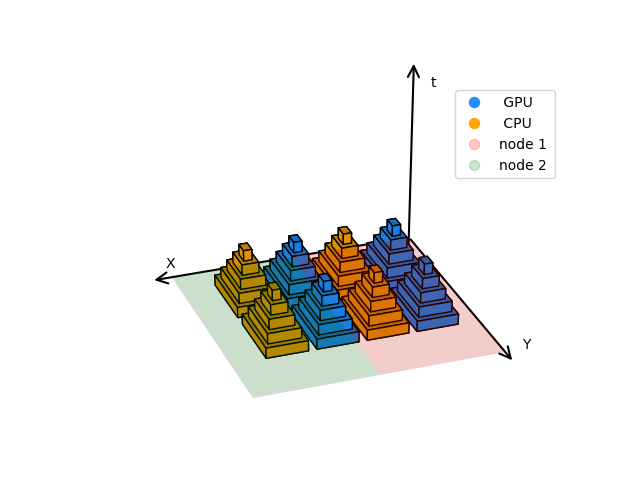
\includegraphics{figs/UpPyramid.png}
    \label{fig:UP}
    \caption{Calculation of the UpPyramid steps (top) and communication of the result (bottom).}
\end{figure}

\par The next step in the process is referred to as the Bridge which occurs independently in each dimension. The number of bridges is equal to twice the number of UpPyramids. The height of the bridges can be determined as
\begin{equation}
  H_{b} = H_{u}-1.
\end{equation}
The dimension in which the bridge grows as time passes is the reference dimension for the bridge (e.g. the bridge that becomes larger in the x dimension is refered to as the X-Bridge). To complete the aforementioned communication process, Bridge shifted regions in each dimension are used to copy data from shared memory to local arrays. Each rank then computes both a X-Bridge and Y-Bridge where a very similar GPU and CPU strategy to the UpPyramid is taken for both bridges. The primary difference is that 1 boundary of each bridge grows in lieu of both boundaries shrinking. Interestingly enough, with the given restrictions, the X-Bridge sets are the inverse of the Y-Bridge sets (i.e. the X-Bridge starts with the set that the Y-Bridge ends on). This is beneficial as only one set of swept step indicies needs to be determined in order to obtain the indicies necessary to solve both bridges. Also, the Bridge phase differs in the fact that it will be executed multiple times over through the simulation as needed to obtain a complete solution between the specified initial and final time. After the calculation is completed, each rank copies the bridge values into the shared memory array to begin the next phase.
% Bridge Figure
\begin{figure}[h!]
    \centering
       \includegraphics[trim={2.8cm 0.9cm 0 0},clip]{figs/YBridgig:OCTe.png}}
    \label{fig:BR}
    \caption{Calculation of the Bridge steps (top) and communication of the result (bottom).}
\end{figure}

\par The next phase of the process is the Octahedron which is essentially super position of the DownPyrmaid and UpPyramid. The DownPyramid indicies are also determined during the pre-sweep phase and they are super imposed with the UpPyramid indicies to form the Octahedron indicies.
The height of the DownPyramid can be determined as
\begin{equation}
  H_{d} =  H_{u}-1
\end{equation}
The height of the Octahedron $H_o$ is then a sum of $H_u$ and $H_d$. The DownPyramid alway begins with a block that is $2N_{pts}$ and grows by $N_{pts}$ on each boundary with every passing time step. The  start is a natural consequence of removing these points during the UpPyramid phase. It is completed upon passing the top of the previous UpPyramid or Octahedron at which time the next UpPyramid portion of this phase begins. The entire Octahedron is calculated in the same fashion as the UpPyramid on both CPU and GPUs. While the steps are described separately for clarity, they are performed in a single calculation step without communication between ranks. The Octahedron step is also a recursive step which is applied as many times as necessary to complete the desired simulation.

% Octahedron
\begin{figure}[h!]
    \centering
       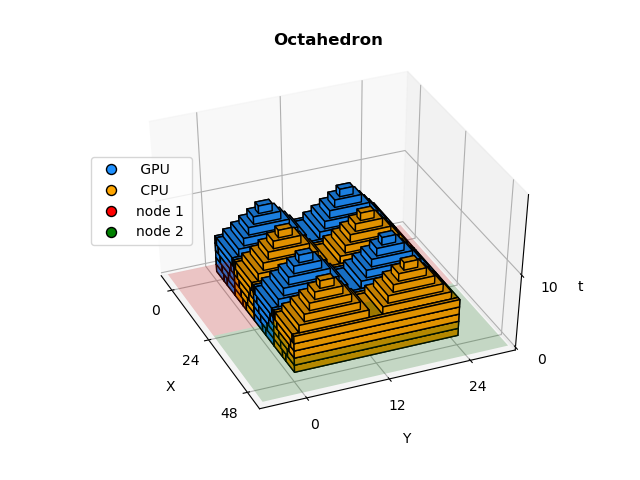
\includegraphics{figs/Octahedron2.png}%[trim={2.8cm 0.9cm 0 0},clip]
    \label{fig:OCT}
    \caption{Calculation of the Octahedron steps (top) and communication of the result (bottom).}
\end{figure}

\par The final phase of the swept process is the DownPyramid which is fairly well described during the Octahedron phase. This is the ending phase of the simulation and is only performed a single time. The strategy is the same as that of the UpPyramid for both the CPU and GPU. The only difference is that all boundaries grow. To summarize the swept phases, the UpPyramid is calculated a single time; The Bridges and Octahedron phases are then repeated until the simulation has reached a value greater than or equal to that of the desired final time.
The actual final time is determined by the number of "swept" steps, ($N_{ss}$) or phases that the simultation is run. This is determined by the given final time and $H_{o}$ which is the minimum time possible of a simulation. It is this way because the simulation only stops after the completion of a phase. These phases occur on both the GPU and CPU with respect to the given affinity. In between each calculation step, a communication step occurs  which consists of shared memory data management and writing out to disk.

\par The shared memory data management of the communication step as well as the writing to disk involve a couple of nuances worth mentioning. It includes shifting of the data which is a strategy implemented for handling boundary blocks in the array. PySweep was implemented with periodic boundary conditions based on the targeted test problems. The boundary blocks of the array form half of the shape it would normally in the direction orthogonal to the boundary (e.g. During the Octahedron phase on the boundary where $x=0$, only half the Octahedron will be formed in the x direction). As expected, the corner will form a fourth of the respective shape. In lieu of added logic for handling these varying shapes, a shifting strategy was developed which allows the majority of the same functions and kernels to be used. The strategy works by writing the data to designated points at the end of the array in each dimension. The shared memory array is exacly $2N_{pts}+b_{s}/2$ points larger in x and y than the given initial conditions array. The shifting of data occurs after every Octahedron phase so that the simulation oscillates between use of its region and shifted region. The boundary points are able to be solved as if they were in the center of a block with this strategy. This strategy comes at the expense of determining the extra regions and storing the extra points in memory. However, the added memory expense of this is minimal due to the strategy for writing to disk and block size restriction. It also mitigates the need for added logic to handle the natural shifting of the shapes and boundaries.

\par PySweep writes to disk after every Octahedron step as it is the ideal time. The code uses parallel HDF5 (h5py) so that each rank can write it's region to disk independently of other ranks. The shared memory array is the height of an Octahedron in time plus the order of the time scheme so that the intermediate steps of the scheme may be used for future steps if necessary. The first $H_{u}$ steps following the $O_{ts}$ steps are written to disk if the step completes the cycle of the specific time scheme (i.e. it is the final step in the time scheme and the values are the desired result). The data is then shifted down in the time dimensions of the array and so that the next phase can be calculated from the region or shifted region. When the write phase occurs after the shifted calculation, the data is shifted back prior to writing so that the writing does not require any conditional statements. This is also necessary for the next calculation step so it is not an added expense.

\par In summary of this swept rule implementation, PySweep is an extensible PDE solver that implements the swept rule in 2 dimensions on heterogeneous architecture. It consists of 2 primary steps which are calculation and communication. The calculation computes points based on a predictable patterns referenced as the phases of the simulation. The communication step is atypical as it does not communicate persay but shifts the perspective of each rank and copies the working data to a local array and then writes it into a shared memory array after the calculation step [MAKE SURE THIS IS ACCURATE, CITE]. This shifting strategy provides simple communication logic at a minimal memory expense. There are multiple phases where both steps occur during the simulation which are the UpPyramid, Bridge (X/Y), Octahedron, and DownPyramid. The solver has a few restrictions based on architecture and implementation which have been previously described. It is currently implemented for periodic boundary conditions only but updating it for other conditions would be fairly straight forward. The solver is also capable of handling given CPU functions and GPU kernels so that it may be used for any desired application that falls within the guidelines presented here. There are some restrictions on the time and spatial schemes \emdash namely that the spatial stencil\emdash but it would be fairly straight forward to handle other cases. PySweep could certainly be further optimized but it is presently sufficient to test and determine the performance capabilities of the 2 dimensional heterogeneous swept rule in comparison to a traditional solver.

\section{Testing}
This implementation of the swept rule was tested against a standard heterogeneous solver (i.e. communicates every time step). This solver uses the same functions provided to the swept solver as well as the same decomposition strategies. The only difference in decomposition is that the standard solver does not break the CPU region assigned to each rank into blocks for solving but simply solves all of the points provided. This actually reduces the cost of the standard solution. The standard solver stores less time steps in memory as it is not necessary to store more than the time scheme depends on. The logic to write each time step to the hdf5 array is also simpler. However, it must write more frequently because less time steps are stored. While there are optimizations that could occur for both the swept and standard solvers, it is believed that the standard solver is sufficient to benchmark the swept solver. The code for the standard solver is available in the PySweep GitHub repository.

\par
The swept solver was tested over a range of affinities, block sizes, and array sizes. These tests were performed on the workstation as previously described in the architecture portion of the implementation section [DOUBLE CHECK THIS]. Affinities between 0.5 and 1 were tested. This range was selected as a result of preliminary testing that showed generally GPU affinities of 1 performed the best for both solvers. So, it was of interest to explore lower affinities yet impractical to test a full range from 0 to 1.

\par
The block sizes tested were 8, 12, 16, 24, and 32. The minimum block size was selected to be 8 because it is a limiting case for the 5 point stencil used to solve the compressible Euler equations. (i.e. It is the minimum size to be able to perform the swept rule). Consequently, it is expected to be the worst case scenario. The upper bound was determined by the GPU architecture.

\par
The array sizes selected were 96, 192, 288, 384, and 480. In particular, the array size was very restrictive because of the nature of 2 dimensional problems with the maximum case containing $480^2$ points. So, the sizes were selected such that a solution could be obtained in timely manner yet be representative of the solvers performance.

\par Each of these cases was executed with two GPUs and 16 CPU processes for 250 time steps. The number of time steps was rather arbitrary in this case because of the nature of the swept rule. In theory, it should not take an absurd number of steps to see performance characteristics because the benefit of reduced latency is compounded with each step. (e.g. if $4\,ns$ are saved every swept step than it should be noticeable after a fairly short amount of time). In some cases, where performance was very close more steps were tested ([ADD NUMBER OF TESTED STEPS]) to be certain of any potential speed up.

\section{Results}

\section{Conclusions}

\section{Acknowledgements}

\section*{References}
\bibliographystyle{unsrt}
\bibliography{references}

\end{document}
